% Niveau :      PCSI
% Discipline :  Méca

\begin{exercise}{Bifurcation fourche supercritique}{3}{Sup}
{Mécanique,Ressort}{lelay}

On considère une bille de masse $m$ glissant sans frottement sur un rail (l'axe $Ox$) accrochée par un ressort de raideur $k$ et de longueur à vide $\ell_0$ placé à une distance $a$ du rail.
\begin{questions}
    \questioncours Rappeler la définition de point d'équilibre en mécanique
    \question À votre avis, quel va être le mouvement de la bille ? Comment va-t-il évoluer en fonction des paramètres du problème ?
    \question Par la méthode de votre choix, trouver les points d'équilibre de la bille. Combien y en a-t-il ?
    \question Représenter sur un graphe les points d'équilibres (sous forme adimensionnée $u=x_{eq}/a$) en fonction de $r = \ell_0/a$.
    \question On s'intéresse maintenant à la stabilité de ces points d'équilibre. Rappeler comment déterminer la stabilité d'un point d'équilibre. 
    \begin{parts}
        \part On considère le cas $a > \ell_0$. Combien de points d'équilibre y a-t-il ? Quelle est leur stabilité ?
        \part On considère le cas $a < \ell_0$. Combien de points d'équilibre y a-t-il ? Quelle est leur stabilité ?
        \part Redessiner le graphe $u = f(r)$ en prenant compte de la stabilité des points. Pourquoi appelle-t-on cette bifurcation \textit{fourche} supercritique ?
    \end{parts}
    \uplevel{\slshape Vous pouvez choisir de faire les deux prochaines question dans l'ordre que vous souhaitez.}
    \question\textsf{Le noeud du problème (\emph{Calculatoire})}.
    \begin{parts}
        \part Dans le cas où $\ell_0 = a$, combien y-a-t-il de points d'équilibre ? Sans calcul, ce point d'équilibre est-il stable ? 
        \part Écrire le PFD au premier ordre non nul en $x$ près du point d'équilibre. Connaissez vous une solution à cette équation différentielle ?
        \part Tracer le portrait de phase correspondant à cette équation, en déduire que le point d'équilibre est stable. \\
        \textbf{Rappel :} le portrait de phase d'un système est le graphique représentant la vitesse en fonction de la position pour différentes conditions initiales.
        \part En supposant que initialement on a $x = x_0$ et $\dot x = 0$, exprimer la période des oscillations en fonction des paramètres du problème et de l'intégrale
        \begin{align*}
        I &= \int_{-1}^1\frac{dy}{\sqrt{1-y^4}} \approx 2.62
        \end{align*}
        \part Proposer des valeurs pour $m$, $k$, $a$ et $x_0$ et calculer $T$.
    \end{parts}
    \question\textsf{La théorie des catastrophes.}
    \begin{parts}
        \part On suppose maintenant que le rail est incliné d'un angle $\alpha$ par rapport à l'horizontale. Montrer que l'équation que vérifient les points fixes donne sous forme adimensionnée :
        \begin{align*}
            1+\frac{h}u = \frac{r}{\sqrt{1+u^2}}
        \end{align*}
        où $h$ est une constante à déterminer.
        \part En supposant $u \ll 1$, montrer que cette équation se réduit à $u^3+h = (r-1)u$. En prenant $h \ll 1$, dessiner les graphes des fonctions $u \mapsto u^3+h$ et $u\mapsto (r-1)u$ pour $r > 1$ et $r<1$. 
        \part En déduire l'allure du graphe $u = f(r)$. Qu'est ce qui a changé par rapport à la situation précédente ? 
        \part Pour un $r>1$ donné, représenter l'allure de $u = f(h)$. Pouvez-vous expliquer pourquoi cette bifurcation est \textit{catastrophique} ?
    \end{parts}

\end{questions}
 \plusloin La théorie des bifurcations est une étape importante pour l'étude des objets complexes, par exemple les systèmes physiques modélisés par des équations non linéaires.
    
% \begin{figure}{H}
%     \centering
%     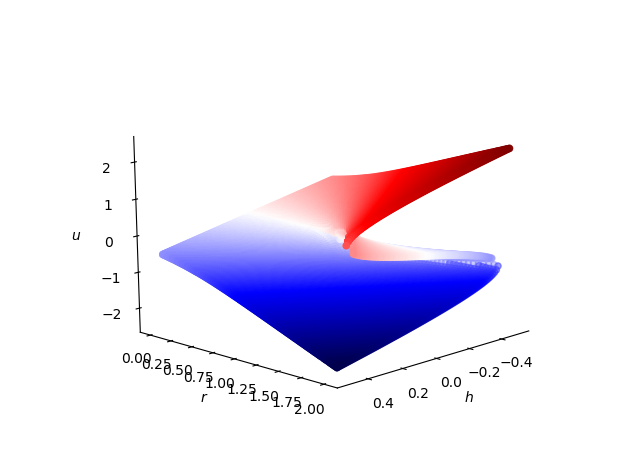
\includegraphics[height=15em]{meca/mecapoint/fourchevraie.png}
%     \caption{Vision pas d'artiste d'une bifurcation fourche supercritique.}
% \end{figure}

% \begin{figure}{H}
%     \centering
%     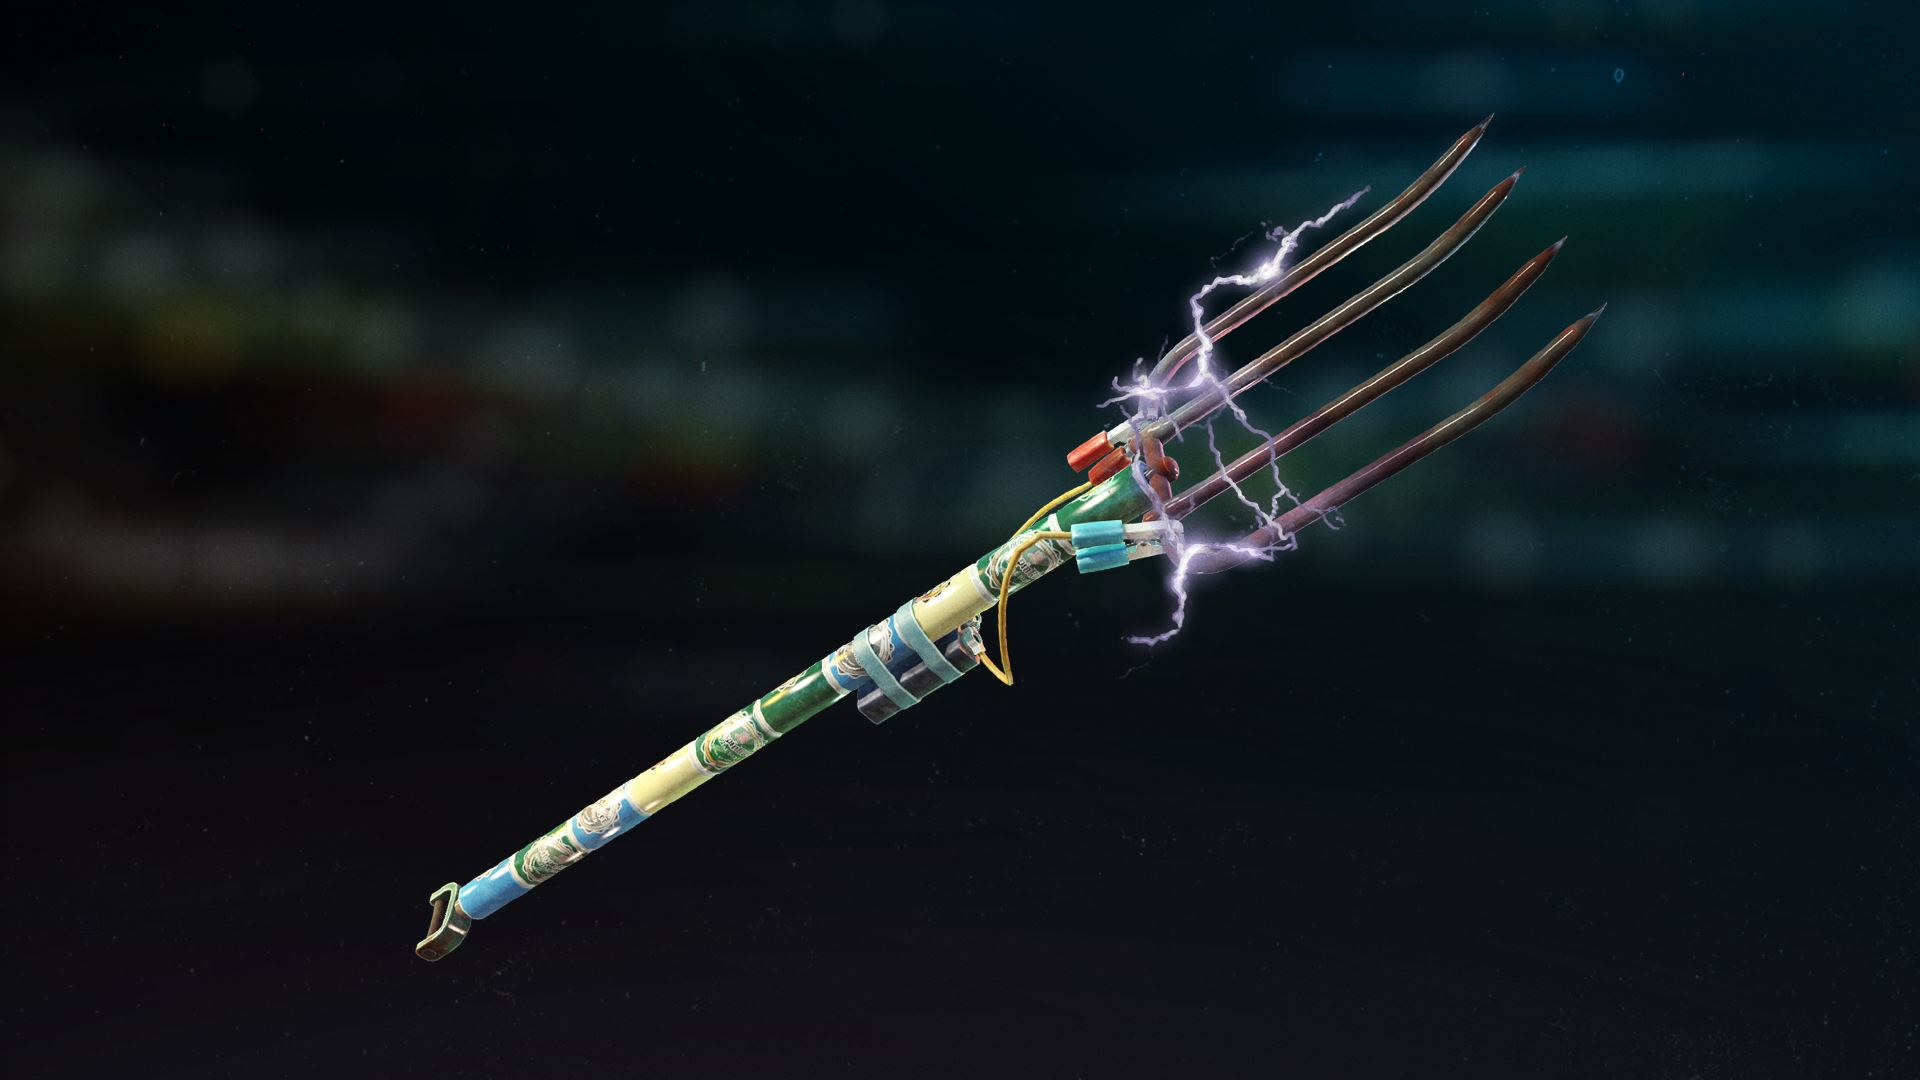
\includegraphics[height=15em]{meca/mecapoint/fourchesupercritique.jpg}%non ! siii ! %gros vilain !
%     \caption{Vision d'artiste d'une fourche supercritique.}
% \end{figure}

\end{exercise}